\section{Ontology Construction and Similarity}
\label{sec1}

After getting job models by the information extraction module, users can search for jobs in the system. In the system, ontology is used as a knowledge base to store knowledge and rules, which could help compare the similarity between different concepts.

\subsection{Ontology Construction}

Before calculating the similarity between concepts, we need to construct the ontology first. Semantic web has been a popular research topic in previous years, and at the same time thousands of domain ontologies have been created~\cite{ding2004swoogle}. A paradigmatic example is WordNet~\cite{fellbaum1998wordnet}, which is a general purpose thesaurus, and contains more than 100,000 general English concepts. ACM has created a poly-hierarchical ontology that can be utilized in semantic web applications~\cite{acm2012class}, but it is mostly used in academic areas. DBpedia~\cite{bizer2009dbpedia} provides structured information from Wikipedia and make this information available on the Web, but its coverage is huge, and most of them is not related to job finding. Currently, there is no domain specific technology ontology built for recruiting purpose.

The domain specific technology ontology for recruiting should include a lot of technical terms, like programming language, programming library, commercial products and so on. Furthermore, there are new techniques invented everyday, so new IT terms will appear continuously. Ding et al.~\cite{ding2002ontology} gave a survey of current ontology generation approaches such as manual, semi-automatic, and automatic. Some aspects of the approaches were discussed in the paper, like the source data, concept extraction methods, ontology representation, and construction tools. Inspired by this paper, we propose a semi-automatic approach to construct the IT skill ontology, which use a pattern matching approach to collect possible technical terms, and use DBpedia to verify the them.

From the observation, we found that sentences with skill requirements in job descriptions always list several skills in the sentence, which is shown in Table ~\ref{tab:skillrequirement}. Based on this character, we propose a bootstrap approach to collect IT terms in job descriptions.  First, we manually collect about fifty terms from job descriptions, and add them to the term list. Then we use our pattern match library to find the sentences that matching the pattern in Table \ref{tab:patterns} from a set of job descriptions. An example of a sentence which matches the pattern is shown in Table \ref{tab:termspattern}. We extract the tokens which match the star symbol from the sentences; these tokens have high probability to be technical terms. Then we could check the tokens in Dbpedia to see whether they are under the categories like software, programming language or any other technical related ones. If they are, we could classify them as terms, and add them to the terms list. After scanning all the sentences in the job description set, the term list will be larger, and we can use the larger term list to start a new iteration of scaning. This process stops when the number of found new terms is below a threshold. The process is shown Figure~\ref{fig:gen_onto}.

\begin{table}[ht]
\caption{Example Sentences in Job Descriptions} % title of Table
\centering % used for centering table
\begin{tabular}{ | p{15cm}  | }
 \hline
    1. A high-level language such as Java, Groovy, Ruby or Python; we use Java and Groovy extensively \newline
    2. HTML5/CSS3/JavaScript, web standards, jQuery or frameworks like AngularJS would be great \newline
    3. HTML CSS and Javascript a must  \newline
    4. Experience with AJAX, XML, XSL, XSLT, CSS, JavaScript, JQuery, HTML and Web Services   \\
 \hline
\end{tabular}
\label{tab:skillrequirement} % is used to refer this table in the text
\end{table}



\begin{table}[ht]
\caption{Patterns to extract terms} % title of Table
\centering % used for centering table
\begin{tabular}{   | p{8cm} |  }
 \hline
     term   , * , *,  term  \\  \hline
     term  , * , *, and  term   \\
 \hline
\end{tabular}
\label{tab:patterns} % is used to refer this table in the text
\end{table}

\begin{table}[ht]
\caption{An example sentence matches the pattern} % title of Table
\centering % used for centering table
\begin{tabular}{   | c | c | c | c |c | c |c | c |c | c |c | c |c | c |  }
 \hline
     Experience & with & TERM & , & *   & , & *   &, & TERM &, & and & *  \\
 \hline
     Experience & with & AJAX & , & XML & , & XSL &, & XSLT &, & and & CSS  \\
 \hline
\end{tabular}
\label{tab:termspattern} % is used to refer this table in the text
\end{table}

For example, we extract the token  ''XSL'', which currently is not in the terms list. We check the word on DBpedia by accessing the URL:http://dbpedia.org/page/XSL. If we can get the XML formatted description of XSL, and any element in ``dcterms:subject'' section has the value which is a technical category,  like ``Programming languages'', ``Markup languages'' and so on, we can indicate that the word is a technical term, and add it to the term list.

\begin{figure}[htbp]
  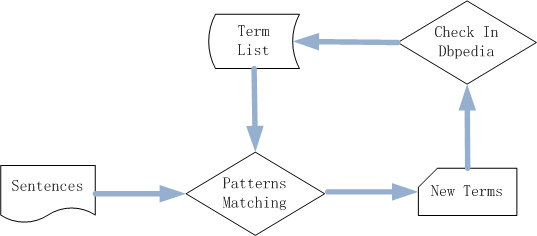
\includegraphics[scale=0.6]{images/genonto.png}
  \caption{Procedure of Finding Technical Terms}
  \label{fig:gen_onto}
\end{figure}

But not all the extracted terms can be verified in DBpedia, because some terms have multiple meanings in English, and the URLs of their DBpedia pages are unpredictable. For example, the word ``Python'' could be an animal name or a programming language.  The meaning of the programming language  has the DBpedia URL http://dbpedia.org/page/Python\_(programming\_language), which is difficult to predict. In this case, we have to check the term manually.  After getting all terms, we use Protege~\cite{noy2001creating}, an open source ontology editor, to edit the domain specific ontology, and saved it in RDF format. Part of the technical ontology is shown in Figure~\ref{fig:ontology_pro}.


\begin{figure}[htbp]
  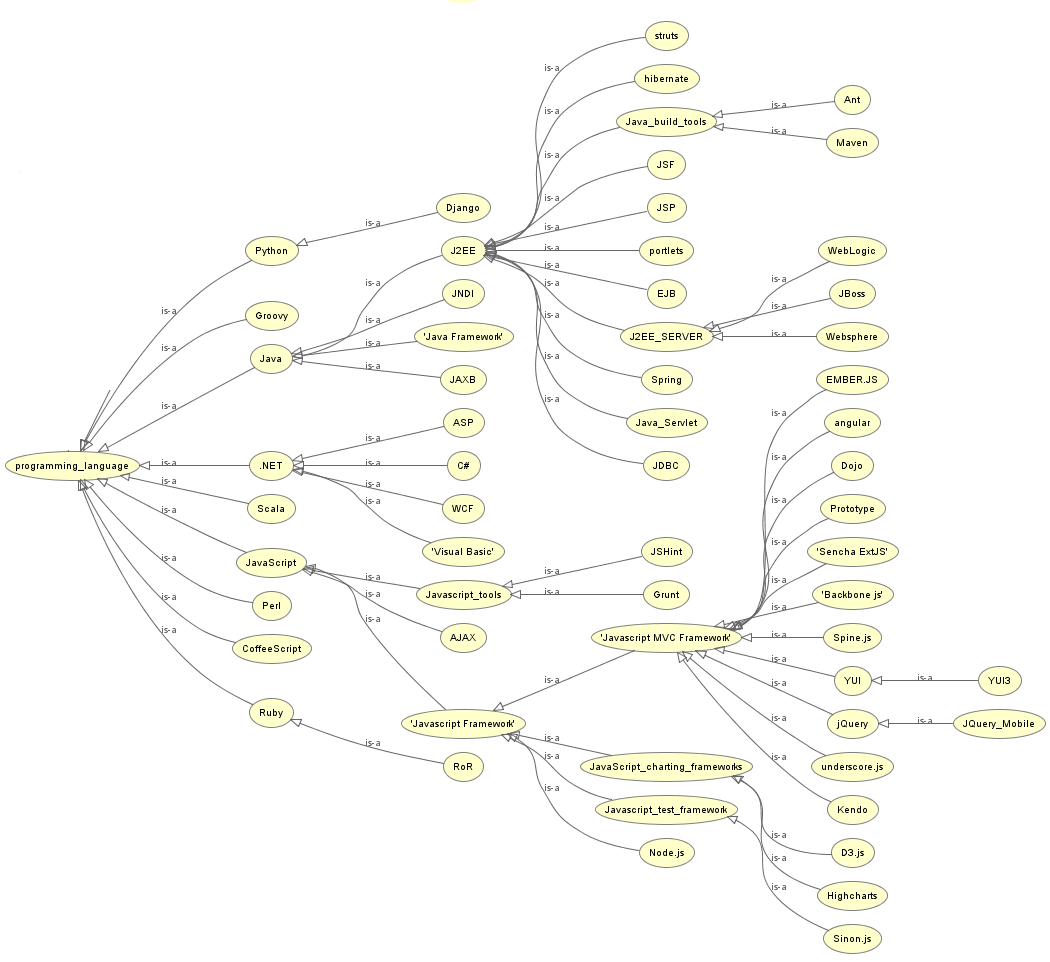
\includegraphics[scale=0.6]{images/ontology_pro.png}
  \caption{Part of Ontology}
  \label{fig:ontology_pro}
\end{figure}

\subsection{Ontology-based semantic similarity}

S{\'a}nchez et al. \cite{sanchez2012ontology} summarized ontology-based similarity assessment into three kinds and gave both advantages and disadvantages of each approach. The three kinds of categories are: Edge-counting approaches, Feature-based measures, and Measures based on Information Content.

In path-based approaches, the ontology is viewed as a directed graph, in which the nodes are the concepts, and the edges are taxonomic relation (e.g. is-a). Rada, et al.~\cite{rada1989development} measure the similarity by the distance of two nodes in the graph. Wu and Palmer~\cite{wu1994verbs} realized that the depth in the taxonomy will impact the similarity measure of two nodes, because the deeper of the nodes are in the tree, the semantic distance is smaller. Based on the same idea, Leacock and Chodorow~\cite{leacock1998combining} also proposed a similarity measure that combined distance   between terms and the depth of the taxonomy. There are some limitations of path-based approaches. First, it only considers the shortest path between concept pairs. When they meet a complex situation like multiple taxonomical inheritance, the accuracy of them will be low. Another problem of the path-based approaches is that they assume that all links in the taxonomy have uniform distance.

Feature based approaches assess the similarity between concepts as a function of their properties. They consider the degree of overlapping between sets of ontological features, like Tversky's model~\cite{tverskyfeatures}, which subtracts the non-common features from common features of two concepts.
Rodr{\'\i}guez and Egenhofer~\cite{rodriguez2003determining} computed similarity by summing the weighted sum of similarities between synsets, features, and neighbour concepts. The feature-based methods consider more semantic knowledge than path-based methods. But only big ontologies/thesauri like Wordnet~\cite{miller1995wordnet} have this kind of information. Ding et al.~\cite{ding2004swoogle} revealed that domain ontologies very occasionally model any semantic feature apart from taxonomical relationship.


Other approaches want to overcome the limitations of edge-counting approaches are Content-based measures. Resnik~\cite{resnik1995using} proposed a similarity measure, which depends on the amount of shared information between two terms. Lin \cite{lin1998information} and Jiang and Conrath \cite{jiang1997semantic} extended Resnik's work. They also considered the IC of each of the evaluated terms, and they proposed that the similarity between two terms should be measured as the ratio between the amount of information needed to state their commonality and the information needed to fully describe them. The are also two disadvantages of the content-based measures. First, the approaches cannot compute the concepts of leave nodes, because they don't have subsumers. Second, if the concepts do not have enough common subsumers, their similarities are hard to be calculated.


\subsection{Statistical-based Ontology Similarity Measure }
In this paper, we proposed a new statistical-based ontology similarity measure. In most job descriptions, they list many skills the positions required. From observation, we found that related skills always exist in the job description simultaneously, and the positions of them are always close, e.g. HTML and CSS are always required together, and appear in the same sentence. We can see from the Table~\ref{tab:skillrequirement}, the closely related concepts are always have short distance. Based on such observation, we give a new statistical-based ontology similarity measure. If two concepts $a$ and $b$ have the same direct hypernym or one  is the hypernym of the other, the similarity between them is given:
$$ S(a,b) = \frac{  N_{a \cap b} / N_{a \cup b} }{avg(\log_2( mindis(d_i,a,b) + 1 ))} $$

The numerator is the ratio of the number of documents in which the two terms exist together $(N_{a \cap b})$ and the number of documents have a least one of them $(N_{a \cup b})$. The denominator is the average $\log$ value of minimum distance $mindis(doc,a,b)$ of the two terms in documents that have them both.

We set the restriction on the position of the two concepts in the ontology, because the position of the concepts in the ontology are based on their technical similarity to others. Similar techniques will be assigned into the same category, so they should share the same hypernym, and one could be an alternative to the other. For example, we put EJB and Hibernate in the same category, because they are both J2EE persistence layer technologies, and both have the O/R mapping concept. If the applicant is familiar one of them, they can master the other very quickly. Another example is Grail and Django, they are both web frameworks and share same web design philosophies, but one of them is designed for Java web application and the other is created for Python web application. If a developer has some some experience with one of them, he/she still need to spend a lot of time to learn the other to overcome the gap between programming languages.

The matrix in Table~\ref{tab:dismatrix1} show the similarity values among of some skills, which is gotten from 500 job descriptions. For example the skill HTML, the most relevant skills in order are CSS, Javascript, and jQuery,  which is the same from the perspective of experienced developers. The other example is Java, the most relevant skill in the matrix is JSP, which is also agree with the general technical knowledge.


\begin{table}

\caption{Similarities of Skills List 1}
\begin{tabular}{ c | c c c c c c   }
 \hline
  Term       &  Java  &  JDBC  & Spring & Hibernate & MySql  & Oracle   \\  \hline
  Java   &   1    & 0.0523 & 0.091  &   0.0458  & 0.0339 & 0.0608    \\  \hline
    JDBC   & 0.0523 &   1    & 0.0525 &   0.0799  & 0.006  & 0.0616   \\  \hline
   Spring  & 0.091  & 0.0525 &   1    &   0.2008  & 0.0194 & 0.0878   \\  \hline
 Hibernate & 0.0458 & 0.0799 & 0.2008 &     1     & 0.0073 & 0.115    \\  \hline
   MySql   & 0.0339 & 0.006  & 0.0194 &   0.0073  &   1    & 0.049    \\  \hline
   Oracle  & 0.0608 & 0.0616 & 0.0878 &   0.115   & 0.049  &   1      \\  \hline
 \hline
\end{tabular}
\label{tab:dismatrix1}
\end{table}


\begin{table}

\caption{Similarities of Skills List 2}
\begin{tabular}{ c | c c c c c c c c }
 \hline
  Term       & Javascript & jQuery &  HTML  &  CSS   &  Java  & Python &  Ruby  &  JSP    \\  \hline
  Javascript &     1      & 0.1981 & 0.2087 & 0.2439 & 0.0665 & 0.0189 & 0.023  & 0.0253   \\
    jQuery   &   0.1981   &   1    & 0.0979 & 0.1328 & 0.0439 & 0.0142 & 0.0266 & 0.0232    \\
     HTML    &   0.2087   & 0.0979 &   1    & 0.3569 & 0.0473 & 0.0175 & 0.023  & 0.0103   \\
     CSS     &   0.2439   & 0.1328 & 0.3569 &   1    & 0.0537 & 0.0153 & 0.0181 & 0.015    \\
     Java    &   0.0665   & 0.0439 & 0.0473 & 0.0537 &   1    & 0.0498 & 0.0287 & 0.075    \\
    Python   &   0.0189   & 0.0142 & 0.0175 & 0.0153 & 0.0498 &   1    & 0.1333 & 0.0025   \\
     Ruby    &   0.023    & 0.0266 & 0.023  & 0.0181 & 0.0287 & 0.1333 &   1    & 0.012    \\
     JSP     &   0.0253   & 0.0232 & 0.0103 & 0.015  & 0.075  & 0.0025 & 0.012  &   1      \\
 \hline
\end{tabular}
\label{tab:dismatrix2}
\end{table}


\subsection{Experiments of Ontology Similarity}

We selected 8 skills from 500 job descriptions; table~\ref{tab:dismatrix2} shows similarity values between these skills. Higher values correspond to greater similarities, so the similarity between one skill and itself is 1. We selected one concept and ranked the other concepts by their similarity values to this concept. Human judges helped rank these concepts by assigning them "relevance scores" so that we can use NDCG to evaluate the effectiveness of our approach.

We use the $ Normalized~Discounted~Cumulative~Gain ( NDCG )$ ~\cite{manning2008introduction} to evaluate the statistical-based similarity. NDCG is an important measure to evaluate the ranked retrieval results, which is the ratio of  Discounted Cumulative Gain ( DCG ) to Ideal Discounted Cumulative Gain ( IDCG ).
 $$ NDCG = \frac {DCG}{IDCG} $$

DCG is the measure of how documents are ranked according to their relevance scores, and IDCG is the DCG value that the documents are strictly sorted by their relevance values.
$$DCG =  \sum_{i=1}^{p} \frac {2^{rel_i} - 1}{\log_2(i+1)} $$

Table~\ref{tab:simcompare1} shows how we evaluate the similarity between the concept ``Javascript'' and other concepts. The first column is a skill name, the second column is its similarity value to ``Javascript'', the third column is its position ranked by the similarity value, and the fourth column is its relevance value given by the judges. The NDCG value for concept Javascript is 0.94, and in Table~\ref{tab:simcompare2},  NDCG value for concept HTML is 0.97. They both hare relative high value.

\begin{table}
\centering
\caption{ Javascript Similarity Evaluation : NDCG = 0.94 }
\begin{tabular}{ | c | c | c  | c |  }
 \hline
    Term     &  Similarity Value  &  Position   & Relevance     \\  \hline
    jQuery   &  0.1981            &      4      &   8        \\
     HTML    &  0.2087            &      3      &   4         \\
     CSS     &  0.2439            &      2      &   3   \\
     Java    &  0.0665            &      5      &   1   \\
    Python   &  0.0189            &      8      &   1   \\
     Ruby    &  0.023             &      7      &   1    \\
     JSP     &  0.0253            &      6      &   2    \\
 \hline
\end{tabular}
\label{tab:simcompare1}
\end{table}


\begin{table}
\centering
\caption{ HTML Similarity Evaluation : NDCG = 0.97 }
\begin{tabular}{ | c | c | c  | c |  }
 \hline
    Term      &  Similarity Value  &  Position   & Relevance     \\  \hline
  Javascript   &  0.2087           &      2      &   3        \\
     jQuery    &  0.0979           &      3      &   3         \\
     CSS     &  0.3569             &      1      &   5   \\
     Java    &  0.0473             &      4      &   1   \\
    Python   &  0.0175             &      6      &   1   \\
     Ruby    &  0.023              &      5      &   1    \\
     JSP     &  0.0103             &      7      &   3    \\
 \hline
\end{tabular}
\label{tab:simcompare2}
\end{table}

